% Setup
\documentclass[a4paper, 11pt]{article}

% Packages
\usepackage{graphicx} % Enables adding figures
\usepackage{subcaption} % Enables figures side-by-side
\usepackage{booktabs} % Makes nicer tables
\usepackage{setspace} % Let's you change the line spacing
\usepackage{hyperref} % Let's you add links (\url{<link>}) and clickable labels to navigate through the document
\usepackage{microtype} % Improves the typesetting of your document by managing better the space between letters, hyphens etc.
\usepackage{parskip} % Improves the spacing between paragraphs
\usepackage{amsfonts} % Adds some math fonts
\usepackage{minted} % Enables syntax highlighting
\usepackage{float} % Enables figures side-by-side

% Brazilian Portuguese
\usepackage[brazil]{babel}
\usepackage[utf8]{inputenc}
\usepackage[T1]{fontenc}

% Geometry
\usepackage[margin=0.75in]{geometry}

% Bibliography
\usepackage[backend=bibtex]{biblatex}
\addbibresource{references.bib}

% Shortcuts
\newcommand{\R}{\mathbb{R}} % Shortcut for the set of real numbers
\newcommand{\eps}{\varepsilon} % Shortcut for the epsilon symbol

% Info
\author{Juan Belieni}
\title{Relatório: implementando o algoritmo de \textit{fuzzy c-means} em Python}
\date{\today}

% Document
\begin{document}

\maketitle

\section{Algoritmo de \textit{fuzzy c-means}}

O algoritmo de \textit{fuzzy c-means}\cite{bartak_jastrzebska_2022} é um algoritmo baseado no tradicional algoritmo de \textit{k-means}.
Nele, cada ponto pode estar associado a mais de um cluster, com uma certa probabilidade, que deve somar 1.

No algoritmo, uma matriz de particionamento $U \in [0, 1]^{C \times P}$ é criada, onde $C$ é o número de clusters e $P$ é o número de pontos.
Cada elemento $u_{ij}$ da matriz representa a probabilidade do $i$-ésimo ponto pertencer ao $j$-ésimo cluster.
Também é definido um vetor $\mathbf v \in \mathbb R^{C \times M}$, que representa os centróides dos clusters, onde $M$ é a dimensão dos pontos.
A clusterização é controlada por um parâmetro $m \in [1, \infty)$, chamado de coeficiente de fuzzificação.

\subsection{Função objetivo}

O \textit{fuzzy c-means} é um algoritmo iterativo, e busca minimizar a função objetivo

\begin{equation}
J = \sum_{i=1}^P \sum_{j=1}^C u_{ij}^m \| \mathbf z_i - \mathbf v_j \|^2,
\end{equation}

onde $\mathbf z_i$ é o $i$-ésimo ponto e $\mathbf v_j$ é o centro do $j$-ésimo cluster.
Para que essa minimização seja feita, o algoritmo define, a cada iteração, novos valores para a matriz de particionamento $U$ e para os centros dos clusters $\mathbf v$ da seguinte forma:

\begin{equation}
u_{ij} = \frac{1}{\sum_{k=1}^C \left( \frac{\| \mathbf z_i - \mathbf v_j \|}{\| \mathbf z_i - \mathbf v_k \|} \right)^{\frac{2}{m-1}}}.
\end{equation}

e

\begin{equation}
\mathbf v_j = \frac{\sum_{i=1}^P u_{ij}^m \mathbf z_i}{\sum_{i=1}^P u_{ij}^m}.
\end{equation}

A cada iteração, o algoritmo verifica se $J^{(k + 1)} - J^k < \eps$, onde $\eps$ é um parâmetro de tolerância.

\section{Implementação}

A implementação do algoritmo de \textit{fuzzy c-means} foi feita em Python, utilizando a biblioteca \textit{numpy} para a manipulação de matrizes e vetores.

\subsection{Métodos auxiliares}

Primeiramente, foi definida a função auxiliar \texttt{J}, que calcula o valor da função objetivo $J$:

\begin{minted}{python}
def J(U: np.ndarray, v: np.ndarray, data: np.ndarray, m: int = 2) -> float:
    return np.sum(
        U ** m,
        * np.linalg.norm(data[:, np.newaxis, :] - v[np.newaxis, :, :], axis=2) ** 2
    )
\end{minted}

\subsection{Método principal}

A função principal do algoritmo é a \texttt{fuzzy\_c\_means}, que recebe como parâmetros a matriz de dados, o número de clusters $C$, o coeficiente de fuzzificação $m$ e a tolerância $\eps$:

\begin{minted}{python}
def fuzzy_c_means(
    data: np.ndarray, C: int, m: int = 2, eps: float = 1e-4
) -> np.ndarray:
    U = np.random.rand(data.shape[0], C)
    U /= U.sum(axis=1, keepdims=True)

    v = np.random.rand(C, data.shape[1]) * data.max()

    J1 = J(U, v, data, m)
    J2 = np.inf

    while np.abs(J1 - J2) > eps:
        for i in range(data.shape[0]):
            for j in range(C):
                d1 = np.linalg.norm(data[i] - v[j])
                d2s = np.linalg.norm(data[i] - v, axis=1)
                U[i, j] = 1 / np.sum(np.power(d1 / d2s, 2 / (m - 1)))

        for j in range(n_clusters):
            s1 = np.sum(U[:, j, np.newaxis] ** m * data, axis=0)
            s2 = np.sum(U[:, j] ** m)
            v[j] = s1 / s2

        J2 = J1
        J1 = J(U, v, data, m)

    return U, v
\end{minted}

\section{Resultados}

A implementação foi testada com a base de dados \textit{World Development Indicators}, presente no \textit{Kaggle}\cite{kaggle_2017}.
Nela, temos dados de diversos indicadores de países ao longo dos anos.
Para a clusterização, foram utilizados alguns indicadores econômicos.

\subsection{Primeira clusterização}

A primeira clusterização foi feita utilizando dois indicadores: PIB per capita e taxa de crescimento do PIB.
Os resultados obtidos são mostrados na figura \ref{fig:cluster-1-plot}.

\begin{figure}[H]
    \centering
    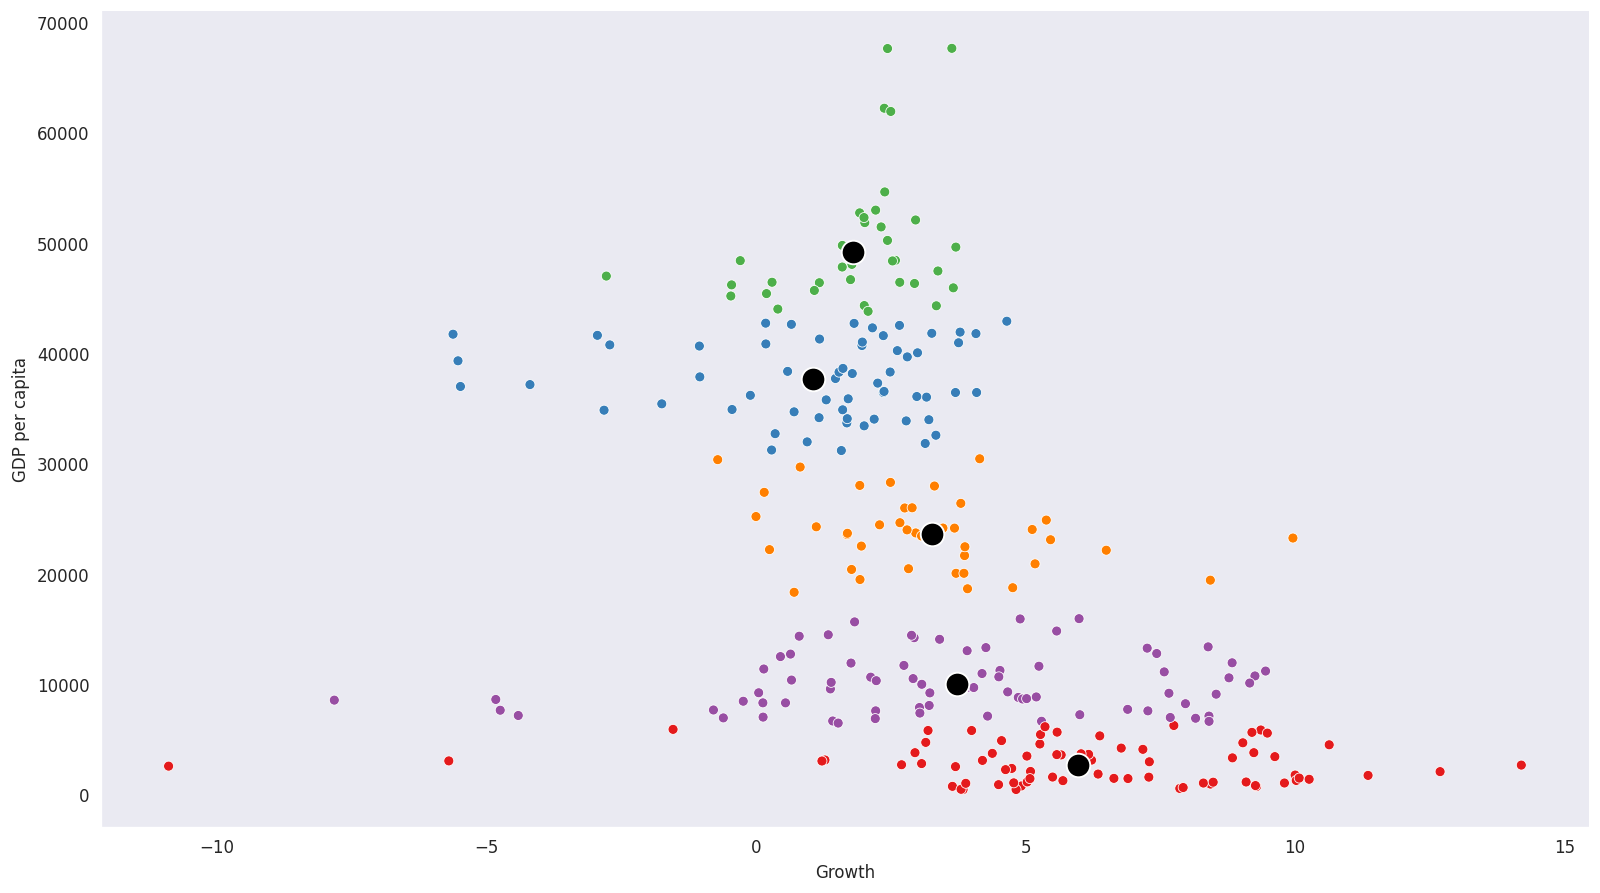
\includegraphics[width=0.8\textwidth]{../images/scatter-cluster.png}
    \caption{Gráfico de dispersão da primeira clusterização}
    \label{fig:cluster-1-plot}
\end{figure}

Além disso, foi possível obter um dendrograma (figura \ref{fig:cluster-1-dendrogram}), que mostra a hierarquia dos clusters, onde a proximidade entre cada país foi calculada utilizando a média do grau de pertencimento de cada país aos clusters.

\begin{figure}[H]
    \centering
    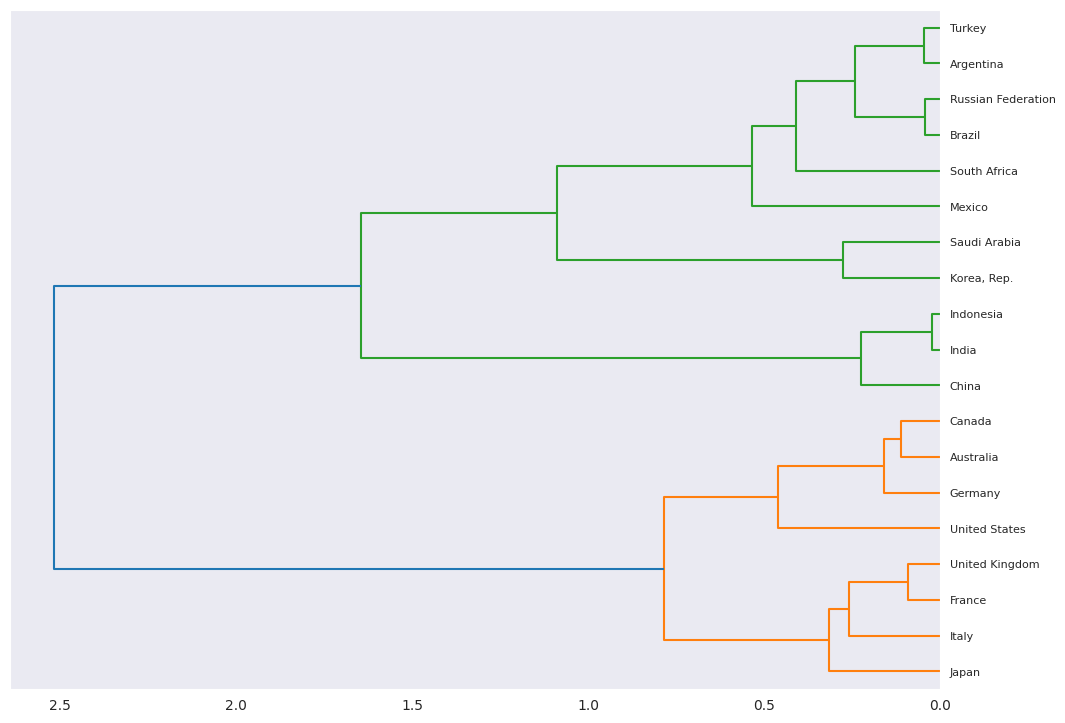
\includegraphics[width=0.8\textwidth]{../images/dendrogram-economy-1.png}
    \caption{Dendrograma da primeira clusterização}
    \label{fig:cluster-1-dendrogram}
\end{figure}

\subsection{Segunda clusterização}

A segunda clusterização foi feita utilizando vários indicadores: PIB per capita, crescimento econômico, inflação, desemprego e crescimento populacional.
Com isso, um segundo dendrograma foi obtido (figura \ref{fig:cluster-2-dendrogram}).

\begin{figure}[H]
    \centering
    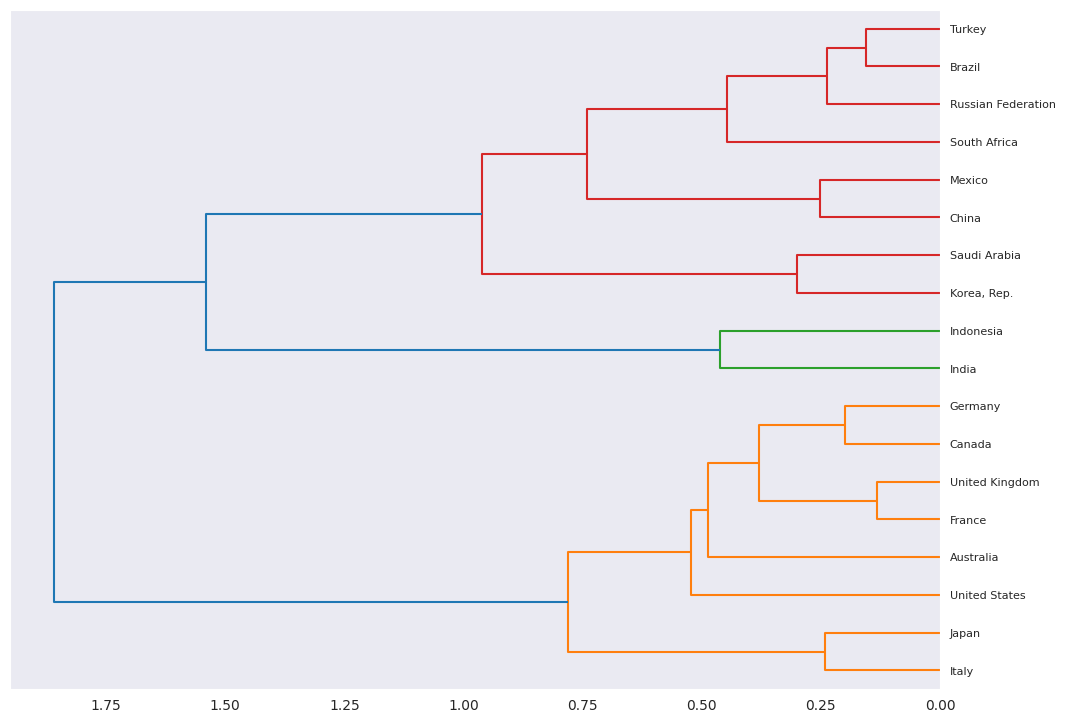
\includegraphics[width=0.8\textwidth]{../images/dendrogram-economy-2.png}
    \caption{Dendrograma da segunda clusterização}
    \label{fig:cluster-2-dendrogram}
\end{figure}

\nocite{*}
\printbibliography

\end{document}
